\chapter{Circuit Schematics}\label{ch:chschematic}
\section{Arduino Pin Connections}
\begin{table}[H]
	\centering
	\begin{tabular}{|l|l|}
		\hline
		Pin of Arduino &Connected to\\
		\hline
		Digital I/O (2) &Trig of HC-SR04\\
		\hline
		Digital I/O (4)  &Echo of HC-SR04\\
		\hline
		Digital I/O (9) &Signal pin of Servo(orange)\\
		\hline
		Vcc &Vcc of HC-SR04 and Servo(Red)\\
		\hline
		GND Pin &GND of HC-SR04 and Servo(Black)\\
		\hline
	\end{tabular}
\end{table}
\section{Breadboard View}
\begin{figure}[H]
	\vfill
	\centering
	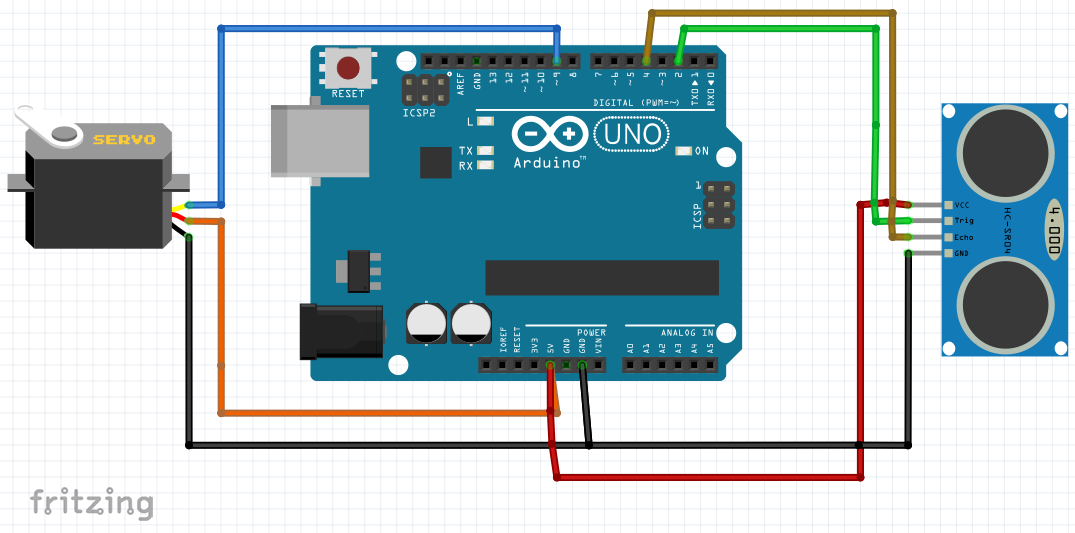
\includegraphics[width=\textwidth]{../Files/bboard}
	\caption{Circuit : Breadboard View}  \label{fig:bboard}
\end{figure}
\section{Schematic view}
\begin{figure}[H]
	\vfill
	\centering
	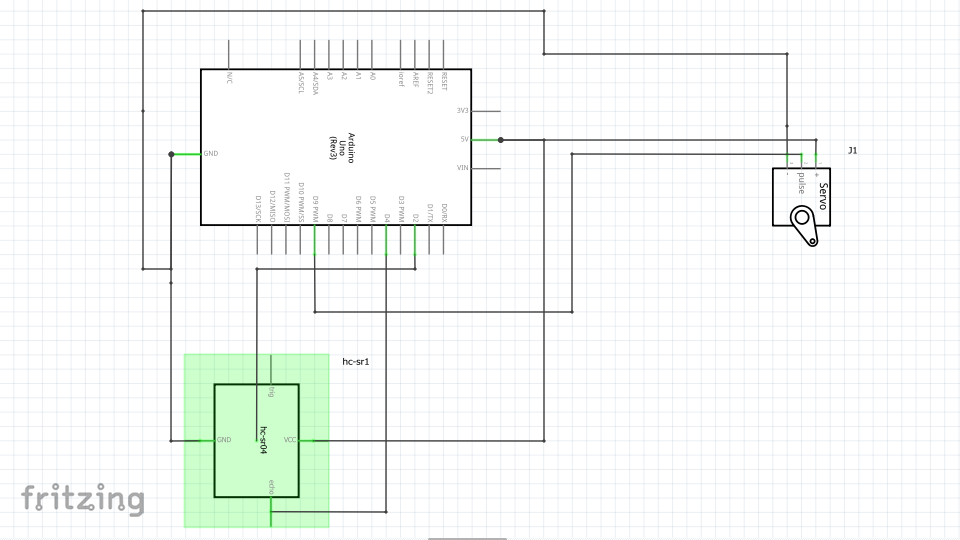
\includegraphics[width=\textwidth]{../Files/schematic}
	\caption{Circuit : Schematic view}  \label{fig:schematics}
\end{figure}
Above circuit schematics were obtained using the Fritzing software.\\
Once we decided the connections, we had to two more steps left before connecting the actual circuit: setting up the\textbf{ Development Environment} and \textbf{Circuit Simulation}.
